\documentclass[11pt,reqno]{amsart}
\usepackage{amsmath,amssymb,booktabs,geometry,microtype,graphicx}
\geometry{letterpaper,margin=1.05in}
\usepackage[colorlinks=true,linkcolor=blue!50!black,citecolor=blue!50!black,urlcolor=blue!50!black]{hyperref}
\usepackage{xcolor}
\input{glyphtounicode}
\pdfgentounicode=1
\newtheorem{theorem}{Theorem}[section]
\newtheorem{lemma}[theorem]{Lemma}
\newtheorem{proposition}[theorem]{Proposition}
\newtheorem{corollary}[theorem]{Corollary}
\theoremstyle{remark}\newtheorem{remark}[theorem]{Remark}
\newcommand{\one}{\mathbf 1}
\newcommand{\Aut}{\operatorname{Aut}_{\pm}}
\newcommand{\HH}{\mathcal H}
\newcommand{\rank}{\operatorname{rank}}
\hypersetup{pdftitle={Rigid woven Hadamard matrices},pdfauthor={Jeffery Kline}}
\title[Rigid woven Hadamard matrices]{Rigid woven Hadamard matrices}
\author{Jeffery Kline}
\date{November 24, 2026\\[3pt]\small Version 0.1.0, \href{https://doi.org/10.5281/zenodo.24507265}{doi:10.5281/zenodo.24507265}}
\begin{document}
\begin{abstract}
Meisner (1992) built Hadamard matrices, \(\pm1\) matrices with orthogonal rows, of order \(N=m^2\) from one of order \(m\): an \(m\times m\) array of rank-one sign blocks whose order and signs can be chosen freely. We prove three results about these matrices and about a second construction, introduced here, of order \(N=4h^2\), in which a transversal design with four groups lets each local sign vector serve four blocks. First, a typical output reveals which of its rows and columns came from each block, so every equivalence must respect the blocks. As a result, all but a fraction \(o(1)\) of the outputs are rigid: their only signed row and column symmetries are the identity and the negation of everything. Second, we count them: for each fixed input, up to signed permutations and transposition, the rigid outputs form \(C\) classes with \(\log C=N\log N-cN+O(\sqrt N\log^2N)\), where \(c=2-\log2\) for Meisner's square and \(c=2+\tfrac18\log2\) for four groups. At order 1600, one design and one matrix of order 20 give more than \(10^{1514}\) rigid regular classes. Third, a rank argument shows why such block constructions need orders divisible by 16: at orders \(N\equiv4\pmod 8\), every partition of a Hadamard matrix into rank-one blocks with no part of size one has all parts of size two, as in the Paley II matrices. The constructions give no new orders.
\end{abstract}
\maketitle

\section{The results}
A real Hadamard matrix \(H\) of order \(N\) has entries in \(\{\pm1\}\) and satisfies \(HH^T=NI\). Write \(\HH(m)\) for existence at order \(m\). We call a matrix regular when all row and column sums are \(\sqrt N\), allowing a change of signs to obtain such a representative where specified. A Bush-type matrix of order \(m^2\) has an \(m\)-by-\(m\) array of square blocks of side \(m\), all diagonal blocks equal to \(J_m\), and all other blocks with zero row and column sums. We allow nonsymmetric Bush-type matrices.

A signed permutation acts by permuting coordinates and negating selected ones. Two matrices are equivalent if one has the form \(UHV^T\) or \(UH^TV^T\) for signed permutations \(U,V\). We call \(H\) \emph{rigid} if the side-preserving group \(\Aut(H)=\{(U,V):UHV^T=H\}\) consists of \((I,I)\) and \((-I,-I)\). Thus the only surviving operation negates all rows and all columns, which leaves the matrix unchanged. Transposition is included when counting classes. All logarithms in the estimates are natural.

Meisner \cite{meisner} gave the square construction as a special case of his order-\(a^2v\) construction. It is also Craigen's weave with the all-ones pattern \cite{craigen}. Choose one normalized local matrix and fix the all-one directions on the diagonal. Permuting and signing its other directions independently gives the Bush ensemble defined in Section~\ref{sec:construction}.

\begin{theorem}[Meisner's square]\label{th:main}
Fix a real Hadamard matrix \(A\) of order \(m\equiv0\bmod4\), normalized for the Bush ensemble, and put \(N=m^2\). As \(m\) tends to infinity through such orders, a fraction \(1-o(1)\) of its Bush labellings have recoverable row and column fibres and give rigid matrices, uniformly in \(A\). Writing \(C_{\rm B}^{\rm rig}\) for their number of classes, we have
\[
 \log C_{\rm B}^{\rm rig}=N\log N-(2-\log2)N+O(\sqrt N\log^2 N).
\]
The same two terms hold for the unrestricted square ensemble. In particular, for all sufficiently large such \(m\) the Bush ensemble gives at least \(\exp(N\log N-(2-\log2)N-O(\sqrt N\log^2N))\) rigid classes. This theorem gives no finite cutoff: at \(m=4\) the outputs from the Sylvester input are not rigid.
\end{theorem}

\begin{theorem}[Four groups]\label{th:four}
Fix an order-\(h\) real Hadamard matrix and a four-group transversal design with the line involution specified in Section~\ref{sec:construction}. Put \(N=4h^2\). Every labelling has a Bush-type regular representative. For a proportion \(1-o(1)\) of labellings as \(h\) grows, the point fibres on both sides can be recovered and the matrix is rigid. The corresponding number of classes satisfies
\[
 \log C_4^{\rm rig}=N\log N-\bigl(2+\tfrac18\log2\bigr)N
                      +O(\sqrt N\log^2 N).
\]
For \(h=20\) one fixed design and the Paley matrix give more than \(10^{1514}\) inequivalent rigid regular matrices.
\end{theorem}

The proofs have three parts. A graph on the local basis labels gives exactly the number of labellings of each raw matrix. Products of four physical rows then recover the hidden point partitions (Figure~\ref{fig:recovery}). Finally, recovery constrains equivalence to permuting points and preserving local Hadamard directions. The last step alone cannot establish rigidity: even with all points fixed there can be signed symmetries within their fibres. We treat that kernel separately for each pattern. The finite bound in Theorem~\ref{th:four} uses a stronger arithmetic test at \(h\equiv4\bmod8\). The third result, Theorem~\ref{th:tworank}, concerns any partition of a Hadamard matrix of order \(N\) into blocks of rank one: the numbers of row and column parts sum to at least \(N\) when \(N\equiv4\pmod 8\), and to at least \(N/2+1\) when \(N\equiv8\pmod{16}\). Section~\ref{sec:sizetwo} shows that the first bound is attained.

\section{Two constructions from local bases}\label{sec:construction}
A \emph{point fibre} is the set of physical rows, or columns, contributed by one local matrix. A \emph{port} is a slot at that point to which one of its basis directions is assigned. A flag is the pair consisting of a point and one of its ports. If the tile at a row point \(x\) and column point \(y\) is
\[
 H_{xy}=\epsilon_{xy}f_{x,p}g_{y,q}^{T},
 \qquad \epsilon_{xy}\in\{\pm1\},
\]
the construction joins row flag \((x,p)\) to column flag \((y,q)\). The coefficient, the joins and the unsigned local bases constitute the fixed input. The ordering and signs of their directions are the labelling. The graph of joins is bipartite.

For fibres of common size \(d\), let \(\widehat F,\widehat G\) be block diagonal with the labelled sign bases divided by \(\sqrt d\). Then \(W=\widehat F^T H\widehat G\) has precisely one entry \(\epsilon_{xy}d\) in each point-pair tile. This normalization matters: in Meisner's square \(W/m\) is a signed permutation. In either example a displayed flag matrix with \(WW^T=NI\) gives a Hadamard matrix after the two orthogonal changes of basis.

\subsection{Meisner's square}
Use \(m\) row points and \(m\) column points. At row point \(i\) assign column \(p_i(j)\) of \(A\) to the tile facing \(j\); at column point \(j\) assign row \(p'_j(i)\) of \(A\) to the tile facing \(i\). In physical coordinates this gives
\[
 H_{(i,e),(j,r)}
 =s_i(j)t_j(i)\,A_{e,p_i(j)} A_{p'_j(i),r}.
\]
For distinct \(i,i'\) the inner sum over \(r\) vanishes by row orthogonality of \(A\). For \(i=i'\) the remaining sum over \(j\) gives \(m^2\delta_{ee'}\). Thus this is Hadamard for any port signs. In the unrestricted ensemble the \(2m\) permutations and their sign vectors are uniform and independent. In the Bush ensemble take \(p_i(i)=p'_i(i)=1\) and both diagonal signs \(+1\). The diagonal tiles are \(J_m\), and each off-diagonal factor is balanced, giving zero margins and regularity.

\subsection{Four groups and a line involution}
Take four groups of \(h\) points, with \(h^2\) lines meeting each group once. Every pair in different groups lies on a unique line. Write \(\ell_i(L)\) for the group-\(i\) point of \(L\). We require an involution \(\pi\) of the lines for which
\[
 L\longmapsto(\ell_i(L),\ell_i(\pi L))
\]
lists all ordered pairs in group \(i\) exactly once, for each \(i\). Index the flags by \((i,L)\). At each row point use columns of \(A^T\) and at each column point columns of \(A\), assigning independent signed permutations to the \(h\) incident lines on each side. With \(\Pi\) the matrix of \(\pi\), take
\[
 K=\begin{pmatrix}0&1&1&1\\-1&0&1&-1\\-1&-1&0&1\\-1&1&-1&0\end{pmatrix},
 \qquad W=h(K\otimes I+I\otimes\Pi).
\]
The summands inside the parentheses commute. One is skew with Gram \(3I\), the other symmetric with square \(I\). Their cross terms cancel and \(WW^T=4h^2I\). At two external points the unique common line supplies the sole join. At two points of one group the ordered-pair condition gives the sole join, including at repeated points. Hence every physical tile is a sign outer product. Each port is used four times.

At a point \(x\), the unique line realizing the pair \((x,x)\) must be fixed, since its image under \(\pi\) realizes the same pair. Thus \(h\) fixed lines partition the points. Let \(z=(-1,1,1,1)^T\), so \((I+K)z=2\one\). At a group-\(i\) column point take as signing vector \(z_i\) times its fixed-line column; at the corresponding row point take its fixed-line column. The first basis change concentrates the input on fixed flags, on which \(W\) acts by \(h(I+K)\). The second basis change produces \(2h\) times the row signing vector. Signing both sides gives row sums \(2h\), and orthogonality gives the same column sums.

On one fixed line the regularized tiles are constant with signs \((I+K)\operatorname{diag}(z)\). Each row and column of this order-four pattern has a single minus. Pair its rows, assigning each pair the two columns avoiding their minus signs. This makes two diagonal all-plus blocks of side \(2h\) and leaves balanced off-diagonal blocks. Between distinct fixed lines both factors of each regularized tile are balanced by orthogonality to their fixed columns. Together the lines therefore give a Bush partition with \(2h\) blocks of side \(2h\). Taking negative entries as incidences gives a Menon design with parameters \((4h^2,2h^2-h,h^2-h)\); a design automorphism preserves the regular matrix by permuting rows and columns.

For explicit inputs over \(\mathbb F_q\), let lines be \((a,b)\), let \(\pi\) exchange \(a,b\), and take four distinct linear forms up to scalar, excluding eigendirections of the exchange. Distinct forms determine an external join, and each form and its exchanged form determine an internal ordered pair. The projective line has \(q+1\) directions; one is forbidden in characteristic two and two in odd characteristic. Thus \(q\ge4\) even or \(q\ge5\) odd suffices. Coordinatewise products preserve both bijections. At \(h=20\) use \(\mathbb F_4\times\mathbb F_5\) and an order-20 Hadamard from Paley at 19 \cite{paley}. More generally \(h=p+1\) works for every prime \(p\equiv7\bmod12\). Its \(2\)-part is at least four and every odd prime factor is at least five. By the prime number theorem in progressions this subfamily supplies asymptotically \(\sqrt X/(4\log X)\) orders through \(X\). Together with \(4h^2\le X\) this gives \(X^{1/2+o(1)}\) distinct supplied orders.

\section{Exact equality and multiplicity under equivalence}\label{sec:gauge}
\begin{lemma}[Gauge of a labelled weave]\label{lem:gauge}
Fix one port at each end of each tile, with one join per point pair, all ports used, and pairwise distinct projective basis directions at each point. Two unrestricted labellings give the same raw matrix precisely when all port permutations agree and their sign ratios are constant on each connected component of the flag graph, on both sides. Each component contributes a factor two. In an ensemble with pinned signs the components meeting a pinned flag contribute a factor one.
\end{lemma}
\begin{proof}
Equality of two outer products of sign vectors identifies the first factors up to a sign and the second factors up to that same sign. Applying this on every tile identifies the basis direction at every port, hence its permutation. The residual ratios at the two ends of an edge must agree. They are constant on connected components, and conversely changing both ends in this way preserves every entry. The choice is free on unpinned components.
\end{proof}

The square has a perfect matching of flags. The four-group graph on one line contains \(K_{4,4}\) minus a matching, which is connected. Its remaining edges join a line to its image under \(\pi\). Thus its components are the \(\pi\)-orbits, numbering \(c=h+(h^2-h)/2\). The exact distinct-output counts are
\begin{align}
 D_{\rm M}&=2^{m^2}(m!)^{2m},&
 D_{\rm B}&=2^{m^2-m}((m-1)!)^{2m},\label{eq:dm}\\
 D_4&=(2^h h!)^{8h}/2^{(h^2+h)/2}.\label{eq:d4}
\end{align}
Here \(D_4\) counts \(\widehat F W\widehat G^T\) before the signing that makes it regular. Regularization preserves each equivalence class. A whole-point sign flip can change the raw matrix and leave its regular representative identical. Conversely, a simultaneous flag flip on a fixed-line component can change the regular representative attached to a labelling giving the same raw matrix. Equation~\eqref{eq:d4} is used only in the raw ensemble.

\begin{lemma}[Cost of equivalence]\label{lem:mult}
Suppose the point fibres on both sides of a labelled output are recovered by a rule equivariant under signed permutations. For \(b\) points on each side, if every local frame admits at most \(a\) signed coordinate permutations preserving its set of projective directions, the number of recoverable distinct outputs in its side-preserving class, itself included, is at most \((b!)^2a^{2b}\). Each side-reversing comparison costs at most another factor two in counting classes. If whole-point flips are allowed at all \(2b\) point occurrences, each class contains at least \(2^{2b-1}\) distinct raw outputs.
\end{lemma}
\begin{proof}
An equivalence on recovered matrices permutes the two sets of points and acts within each fibre. The outer products show that each local operation carries all the projective directions of the source frame to those of the target frame. In these fixed-base ensembles the set of allowable operations is its frame stabilizer, or a coset of the same size between two frames. Specifying the point maps and these local operations determines the target matrix. A transpose class contains at most two side-preserving classes. Finally, the \(2^{2b}\) whole-point sign choices give the same matrix only in complementary pairs: every row point meets every column point in a nonzero tile.
\end{proof}

For a local sign Hadamard of order \(d\), set \(r=\lceil2\log_2 d\rceil+2\) and \(a(d)=(2d)^r\). A random list of \(r\) coordinates fails to distinguish a given pair of column rays with probability \(2^{1-r}\). A union bound gives a distinguishing list. Specifying its signed preimages determines the action on all columns, including their signs, and hence the entire signed coordinate operation. Thus \(a(d)\) bounds the full local stabilizer for either orientation of a basis.

The method has the following conditional form. It separates three properties that must be checked in an application.
\begin{proposition}[Criterion for counting rigid outputs]\label{prop:criterion}
In a sequence of fixed-input ensembles as above, suppose \(b,d=O(\sqrt N)\), every raw output has the same number of labellings, and, with probability \(1-o(1)\), (i) an equivariant decoder recovers both point partitions, (ii) no nonidentity pair of point permutations lifts to a signed automorphism, and (iii) the kernel fixing all points consists of simultaneous scalars. If \(D\) is the exact raw output count and \(C^{\rm rig}\) counts classes, transposes identified, containing an output with properties (i)--(iii), then
\[
 \log D-O(\sqrt N\log^2 N)\ \le\ \log C^{\rm rig}\ \le\ \log D.
\]
\end{proposition}
\begin{proof}
Equal-size labelling fibres give at least \((1-o(1))D\) distinct outputs with the three properties. The last two properties give rigidity. Lemma~\ref{lem:mult} and the distinguishing-coordinate bound give the lower estimate after division by \(2(b!)^2a(d)^{2b}\). The upper estimate counts all raw outputs.
\end{proof}
For the two patterns, the independence estimate for moved points and the two different kernel estimates below supply (ii) and (iii). Recovery alone leaves point permutations possible.

\section{Recovering the fibres from the entries}\label{sec:recover}
\begin{figure}[t]
\centering
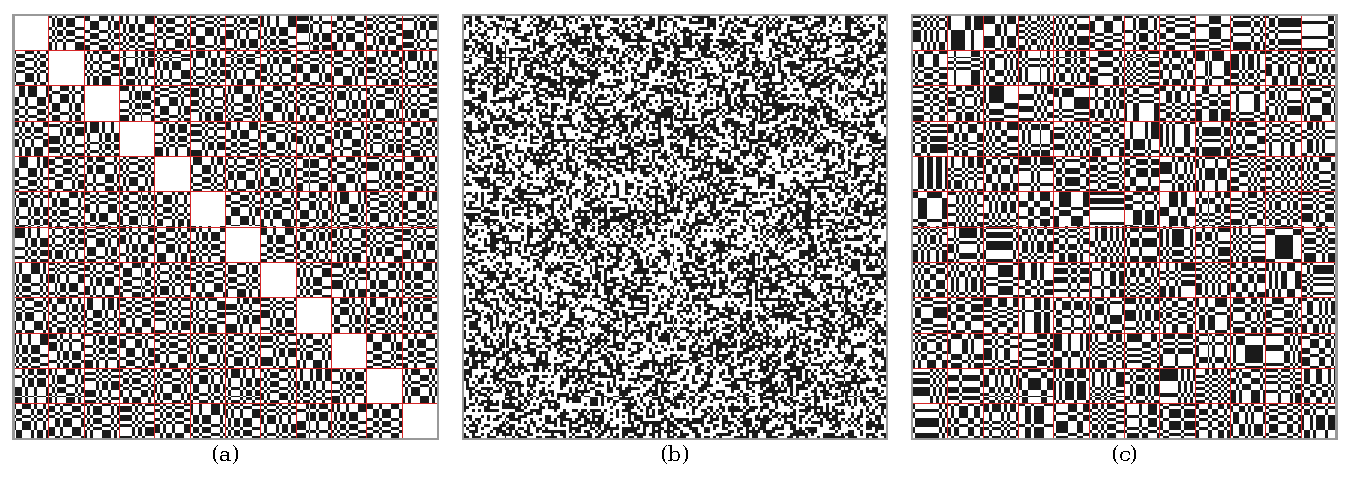
\includegraphics[width=\textwidth]{fig-recovery.pdf}
\caption{Recovering the blocks of a Meisner square from its entries. Black is \(-1\), white \(+1\). (a)~A Bush-type square of order \(N=144\) (\(m=12\)), built from the Paley-type Hadamard matrix of order~12, with its \(12\times12\) grid of rank-one blocks. (b)~The same matrix after a random signed permutation of its rows and columns. (c)~Matrix~(b) with its rows and columns re-sorted into the fibres found by the divisibility test in the proof of Proposition~\ref{prop:recovery}, which reads only the entries of~(b). The test finds all 12 row fibres and all 12 column fibres, so every block is again of rank one. It does not recover the order of the fibres, the order within a fibre, or the signs. These are exactly what the disguise changed, and (b) alone cannot reveal them; so (c) is equivalent to (a) but not equal to it.
Cautions. (i)~The theorems are asymptotic. The figure illustrates recovery and makes no rigidity claim for this matrix. (ii)~Proposition~\ref{prop:recovery} chooses between two tests, and at this small order the choice goes wrong: some quartets that mix two fibres reach \(N/2\), which selects the large-quartet test, and that test finds 144 column fibres instead of 12. The figure therefore applies the divisibility test directly. (iii)~The divisibility test fails on Sylvester inputs: at order 64, where Sylvester's matrix is the only possible input, it relates all 2016 pairs of rows instead of the 224 true pairs. (iv)~The test evaluates about \(N^4/4\) sums of fourfold products, and its success here was checked against the hidden fibres for one random seed only. The script \texttt{figure\_recovery.py} draws the figure and checks each statement in this caption.}
\label{fig:recovery}
\end{figure}
For sign rows \(u,v,w,z\) let \(D(u,v,w,z)=\sum_k u_kv_kw_kz_k\). Its absolute value is invariant under signed equivalence of the rows and columns. Row products from a single fibre are constant on every opposite fibre. For rows at different points the product is nonconstant on a fibre seeing two different ports, because distinct local Hadamard directions are orthogonal. In the square, every opposite point separates two distinct row points. In the four-group geometry at least \(h-1\) points in any group external to the two points separate them: two points in different groups share just one line, and two in one group share none. The assertions are symmetric in the two sides. Consequently either partition, once known, determines the other.

\begin{proposition}\label{prop:recovery}
In both ensembles of the square and in the four-group construction, a rule depending only on the matrix entries recovers both point partitions with probability \(1-o(1)\), uniformly in the allowed fixed inputs.
\end{proposition}
\begin{proof}
Use \(d=m\) or \(h\) for the local order. In the square the relevant quartet correlations are those of rows of \(A\): these are both the local physical rows on the left and the port directions on the right. In the four-group construction use columns of \(A\), by the choice \(A^T\) on the left. Write \(b\) for the number of points per side, and \(N=bd\).

\emph{Large quartets.} If a local quartet has \(|D|\ge d/2\), its physical copy at each row point has global absolute sum \(b|D|\ge N/2\). For a mixed quartet with odd multiplicity at some point, conditional on all other variables its sum has the form \(\sum_p s_pc_p\) with \(d\) independent fair signs and \(|c_p|\le b\). The exponential bound is \(2e^{-d/8}\) at threshold \(N/2\). In the remaining mixed pattern, two rows at one point and two at another, the product at the first point is a uniformly permuted balanced word independent of the other point. Conditioning fair signs to be balanced costs at most \(d+1\). In the Bush model one diagonal entry is pinned; remove that summand and condition on the corresponding composition on \(m-1\) slots. The bounds become \(2e^{-m/8+O(1)}\) and \(O(m)e^{-m/8+O(1)}\), respectively. A union bound over fewer than \(N^4\) quartets makes the probability of any mixed threshold quartet \(o(1)\).

Take all row pairs in threshold quartets, and list their products at each column. Columns in the same fibre have identical lists on the preceding event. At each separating row point the deterministic large quartet supplies two rows whose product is a randomly permuted balanced word. At two distinct port positions the chance of equal values is \((d-2)/(2(d-1))<1/2\). There are at least \(h-1\) independent probes in four groups, and \(m\) in the unrestricted square. In the Bush square discard the two possible diagonal probes; on the remaining positions the pinned balanced word has collision probability at most \(1/2\). A union bound over opposite point pairs gives \(o(1)\). These estimates bound the unconditional chance of a missed separation, so there is no conditioning on which pairs happened to be detected. Equal lists now give the column partition.

\emph{Small quartets.} Suppose every distinct local quartet has \(|D|<d/2\). Relate two physical rows when every extension by two further distinct rows has fourth sum divisible by \(d\). A true pair passes because each column fibre contributes \(0\) or \(\pm d\). For a false pair choose a separating column point \(y\), with distinct ports \(a,b'\). Choose one auxiliary physical row facing each other eligible port \(c\) at \(y\). For four groups take these rows from distinct points in a row group different from the original two. In the square take one from point \(c\) and omit the diagonal port \(y\) as well. Choices can be made before the auxiliary port signs are exposed.

On the eligible ports join \(c,c'\) when the local quartet \(D_{ab'cc'}\) is nonzero. In four groups the product of columns \(a,b',c\) is orthogonal to those three and has a nonzero coefficient on another basis column. In the square we also excluded \(y\). Parseval gives
\[
 \sum_{c'} D_{ab'cc'}^2=d^2.
\]
The three repeated-index terms vanish; every other coefficient has magnitude strictly less than \(d/2\). At least five coefficients are nonzero, so excluding \(y\) still leaves a neighbour. Thus neither graph has an isolated vertex.

After exposing all variables except the auxiliary signs at \(y\), an edge gives a global fourth sum \(\kappa_{cc'}+\sigma_{cc'}D_{ab'cc'}s_cs_{c'}\), with the first term and coefficient fixed. Since \(0<2|D_{ab'cc'}|<d\), at most one product of signs passes the divisibility test. The products on edges of a forest are independent. A spanning forest has at least \((h-2)/2\) edges in four groups and \((m-3)/2\) in the square. Union bounding the resulting exponentially small false-pair probability over at most \(\binom N2\) pairs recovers the row partition.

The rule is to take the large-quartet branch whenever \emph{any} physical quartet reaches \(N/2\); otherwise take the divisibility branch. In the small-quartet case an incorrect branch requires a mixed threshold quartet. A Sylvester basis with a closed quartet takes the large-quartet branch even if its divisibility test accepts many false pairs. Signed changes of rows multiply a pair's whole list component by one sign, and column signs cancel. All recovery steps therefore commute with signed permutations.
\end{proof}

In the four-group case one can now read the four opposite fibres using any given port: they are exactly those whose tiles have the same projective factor at the recovered point. This is the incidence information used in the count. In the square each direction appears just once.

\section{Rigidity of the two ensembles}\label{sec:rigid}
A recovered automorphism induces permutations \(\alpha,\beta\) of the row and column points. They prescribe all port maps whenever those maps exist, by the incidences just recovered. In the square the row port map is simply \(j\mapsto\beta j\). For any prescribed point action of total support \(s\), expose the independent port permutations successively along each moved cycle. After its first point, each successor permits at most \(a(d)\) permutations since local coordinates must preserve the set of basis directions. Discarding the closing constraint leaves at least \(s/2\) restrictions. Use \(t=d!\) for the unrestricted ensembles and \(t=(m-1)!\) for the Bush square. Summing over all nonidentity actions gives the bound
\[
 \sum_{s\ge2}\bigl(2b\sqrt{a(d)/t}\bigr)^s=o(1).
\]
This is a union over prescribed point actions; recovery failure is accounted for separately.

For the kernel over the identity point action, let \(B\) be a local basis. A signed coordinate permutation fixing every port ray satisfies \(UB=B\operatorname{diag}(e)\). Reading one fixed row shows that \(e\) belongs to a set of at most \(2d\) signed entrywise products of that row with a row of \(B\). Each nonconstant candidate is balanced. A permutation of the port labels permutes the word \(e\); signing the basis columns leaves the candidate set unchanged.

\subsection{Four groups}
Each flag join equates its two endpoint eigenvalue signs. On one line an external path of length three connects row \((i,L)\) to column \((i,L)\) via two other groups. Thus the row and column kernel words at the same physical point agree flag by flag. The two local port permutations there are independent, so the probability of any common nonconstant word is at most \((2h)^2/\binom{h}{h/2}\). Union bound over \(4h\) points. With high probability every point acts by a scalar. The tile between every ordered point pair then forces one common scalar. This proves the rigidity assertion in Theorem~\ref{th:four}.

\subsection{Meisner's square}
The eigenvalue on tile \((i,j)\) defines a sign \(X_{ij}\) common to both ends. Each row of \(X\) belongs to the kernel-word set at a row point, and each column to its independently permuted analogue for the transposed local basis. An individual nonconstant candidate is uniform over balanced words, with one fixed coordinate in the Bush case.

Take \(\delta=1/4\) and let \(H_2\) denote binary entropy to base two. The probability that two candidate nonconstant words from different row points are within \(\delta m\), allowing either sign, is bounded after the union over point pairs and candidate pairs by
\[
 O(m^5)\,2^{(H_2(\delta)-1)m}=o(1).
\]
Indeed a Hamming ball has at most \(2^{mH_2(\delta)}\) words and
\(\binom m{m/2}\ge 2^m/(m+1)\); a pinned coordinate costs a factor of at most two. A constant and a nonconstant word have distance \(m/2\).

Condition on row labellings with this separation property. If all rows of a compatible \(X\) coincide, their common word belongs to two different row-point sets and must be constant. Otherwise two rows differ in at least \(\delta m\) places, so \(X\) has at least \(\delta m\) nonconstant columns. There are at most \((2m)^m\) candidates \(X\) from the row sets. For each one, the chance that the independent column sets accept its specified nonconstant columns is at most \((4m(m+1)2^{-m})^{\delta m}\). The product is \(2^{-\delta m^2+O(m\log m)}\). Thus \(X=J\) or \(-J\) with high probability; every local operator acts by that same scalar. This proves rigidity in Theorem~\ref{th:main}, including the pinned Bush case.

\section{Counting rigid classes and designs}
The equal-size gauge fibres in Lemma~\ref{lem:gauge} transfer a proportion of good labellings directly to a proportion of distinct good outputs. In four groups put \(b=4h\) and \(a=a(h)\). Lemma~\ref{lem:mult} gives
\[
 \frac{(1-o(1))D_4}{2(b!)^2a^{2b}}
 \le C_4^{\rm rig}\le C_4\le \frac{D_4}{2^{2b-1}} .
\]
For the unrestricted square replace \(D_4,b,a\) by \(D_{\rm M},m,a(m)\). For the Bush square use \(D_{\rm B}\) and the upper bound \(D_{\rm B}\) itself; whole-point sign changes need not preserve its pinned diagonal. Substitution of \eqref{eq:dm}--\eqref{eq:d4} and Stirling's formula prove both logarithmic class counts. In particular the equivalence loss for the rigid outputs is at most \(\exp(O(\sqrt N\log^2 N))\). All counts refer to a fixed input at the stated order. The exact integers \(D\) count distinct matrices; the error term concerns classes.

\begin{corollary}[Rigid Hadamard designs]\label{cor:designs}
At every sufficiently large \(N=m^2\) in Theorem~\ref{th:main}, the lower bound there also holds for the number of pairwise nonisomorphic rigid Hadamard designs on \(N-1\) points. Where both \(\HH(m)\) and \(\HH(m^2/8)\) hold, the leading term of the logarithmic lower bound is \(N\log N\), twice that of Merchant's Theorem~5.2.
\end{corollary}
\begin{proof}
Normalize a selected row and column to all pluses, delete them, and use the plus entries of the remaining square as incidences. The resulting symmetric design has parameters \((N-1,N/2-1,N/4-1)\), by row orthogonality. Call it the design associated with the distinguished row and column. A design automorphism extends to an automorphism of the normalized matrix fixing the distinguished row and column. With signed matrix rigidity only the identity permutation can arise. Isomorphic associated designs rebuild equivalent bordered matrices, so inequivalent matrices yield nonisomorphic designs. This applies to every choice of the distinguished coordinates.

Merchant \cite[Theorem~5.2]{merchant} starts with a Hadamard design of order \(n>2\), equivalently \(\HH(4n)\), and obtains at least \((16n-2)!/(2^{10}n^3)\) rigid designs of order \(8n\). In matrix-order notation \(N=32n\); his logarithmic lower bound has leading term \((N/2)\log N\). His additional conclusions concern good blocks, good points and tensor indecomposability. The comparison here concerns the number of rigid designs on the common range. The doubling is asymptotic. At \(N=1600\), where \(\HH(40)\) and \(\HH(200)\) both hold, Merchant's bound with \(n=50\) exceeds \(10^{1962}\) rigid designs, more than the finite count of Theorem~\ref{th:four} implies. \end{proof}
Earlier, Norman \cite{norman73} constructed rigid Hadamard designs. The full text of that paper was not openly accessible at the time of writing; Merchant reports that it gives an infinite family of rigid Hadamard designs from doubled Paley designs.

\section{The finite count at order 1600}\label{sec:finite}
Asymptotic rarity of exceptional labellings does not by itself give a finite example. For \(h\equiv4\bmod8\), \(h\ge20\), every quartet in a local Hadamard supplies a modular constraint, and occasional false pair detections can be tolerated.

\begin{proof}[Proof of the finite assertion of Theorem~\ref{th:four}]
Normalize one of four distinct local columns to all pluses. For the other three columns \(u,v,w\), the number of occurrences of each pattern \((a,b,c)\) is \((h+abcD)/8\), where \(D=\sum uvw\). Thus \(D\equiv4\bmod8\). If \(|D|=h\), one can arrange \(w=uv\); a fifth column would then have zero sum in each of four cells of odd size \(h/4\). Hence \(0<|D|<h\), and \(h\nmid 2D\) since the intermediate possibility \(|D|=h/2\) has the wrong residue. The same holds for row quartets.

Use the divisibility relation from Proposition~\ref{prop:recovery}. Every edge on the \(h-2\) auxiliary ports distinguishes the two sign products, so a spanning tree bounds the chance of a given false pair by \(2^{-(h-3)}\). Here the decoder outputs the partition of this divisibility graph into \(h\)-cliques when that partition is unique. It is not the branch rule of Proposition~\ref{prop:recovery}, which would take the large-quartet branch for the Paley matrix (\(|D|=12\)). The rule depends only on the entries and commutes with signed permutations. The true fibres are cliques of size \(h\). An alternative partition into such cliques has at least two mixed cliques; each uses at least \(h-1\) false edges. By Markov's inequality the probability of failure of uniqueness is at most
\[
 f_h=\frac{\binom{4h}{2}h^2}{2(h-1)2^{h-3}} .
\]
Thus one can tolerate false edges without losing the partition.

For a finite estimate of the action on the \(h\) column rays, record three row coordinates and take ratios against the first coordinate. The four patterns have equal multiplicity \(h/4\). Choosing three ordered preimages, their relative signs and the bijections of the four cells gives
\[
 a_h^{\rm proj}=4h(h-1)(h-2)((h/4)!)^4 .
\]
If a signed local operator fixes every column ray, any nonconstant kernel word multiplies the projective rows in fixed-point-free pairs. Two such pairs then give a quartet of magnitude \(h\), which we just excluded. Thus the full local frame group has size at most \(2a_h^{\rm proj}\).

With \(r_h=4h\sqrt{a_h^{\rm proj}/h!}\), the cycle-exposure bound on both independent point sets is \(g_h\le(1+r_h^2/(1-r_h))^2-1\), omitting support one on each side. At \(h=20\),
\[
 f_{20}<0.254,\qquad
 a_{20}^{\rm proj}=5\,673\,369\,600\,000,\qquad r_{20}<1/8,\qquad g_{20}<0.037 .
\]
In fact the good fraction exceeds \(70\%\) for all admissible \(h\equiv4\bmod8\), \(h\ge20\). The upper bound \(4h^4/((h-1)2^{h-3})\) for \(f_h\) decreases from less than \(0.258\). Also \(r_{h+4}^2/r_h^2=(1+4/h)^2(h+4)^4/[256(h+1)h(h-1)(h-2)]<1\) for \(h\ge20\). At \(h=20\), using only the lower good fraction \(1/2\), the transpose factor two and the exact raw gauge \(2^{210}\), the class count exceeds
\[
 \frac{(2^{20}20!)^{160}}{4(80!)^2(2a_{20}^{\rm proj})^{160}2^{210}}.
\]
The floor has 1515 decimal digits, beginning \(587135898904\). This proves the claimed strict bound.
\end{proof}

The release code constructs one explicit labelling at this order: its \(2\,560\,000\) entries are signs, all row and column sums are \(40\), and all \(1\,279\,200\) pairs of rows are at distance \(800\). Its individual signed automorphism group has not been certified. The rigid count above is an existence statement over the fixed ensemble.

For comparison, pinning only the all-one directions in Meisner's square leaves \(((m-1)!)^{2m}2^{m^2}\) distinct outputs if every tile sign is free. At \(m=40\) this has 4187 digits, compared with 3842 for \(D_4\). One also obtains a finite bound for the positive-diagonal Bush square without generic recovery. Guess one row fibre of a competing labelling in at most \(N^m\) ways. On that fibre, proportional restrictions of columns identify the opposite fibres, because each port there appears once. One recovered column fibre likewise determines the row fibres. After naming points there are at most \((m!)^2(2m\,a_m^{\rm proj})^{2m}\) induced signed coordinate choices, using the elementary \(2m\) bound on each local kernel. Hence
\[
 C_{\rm B}\ \ge\ \frac{D_{\rm B}}{2N^m(m!)^2(2m\,a_m^{\rm proj})^{2m}}>10^{1268}
 \qquad(m=40).
\]
This finite square bound counts classes without a rigidity condition. The lower bounds do not order the actual class counts at \(1600\). At common orders \(m=2h\) the two logarithmic formulas differ by \((9\log2/8)N+O(\sqrt N\log^2 N)\), in favour of Meisner's square.
\section{Order coverage and blocks of rank one}
\subsection{Which orders the method supplies}
Meisner already obtains regular order \(m^2\) from \(\HH(m)\). In the four-group family \(m=2h\) is supplied by doubling the given order-\(h\) Hadamard. An independent symmetric Bush witness follows from Kharaghani's construction as reproduced by Bonato, Holzmann and Kharaghani \cite[Theorem~1]{bhk}. Hence neither theorem settles an existence question at a new order.

More generally, for real local Hadamard bases of possibly unequal orders \(h_x,h_y\), each nonzero entry of the flag matrix at a tile has absolute value \(\sqrt{h_xh_y}\). Its row norm gives
\[
 N=h_x\sum_{y\ \mathrm{faced\ by}\ p}h_y
\]
for every port \(p\) at \(x\). If all fibres on both sides have size at least four, then \(16\mid N\). In particular no such construction with all fibres of size at least four reaches a regular order \(4u^2\) with \(u\) odd. A regular output order is then \((2w)^2\); whenever \(\HH(2w)\) holds, the square construction from that matrix already gives a regular witness at that order. This applies to every order supplied by Theorems~\ref{th:main} and~\ref{th:four}. We do not show that a general construction of this shape needs \(\HH(2w)\).

The divisibility \(16\mid N\) uses real local Hadamard bases. A rank argument removes that hypothesis: it applies to any partition into blocks of rank one, whatever the local inputs or their defects. For a sign matrix \(M\) write \(M=(-1)^{\beta}\) with \(\beta\) a \(0/1\) matrix, and let \(\operatorname{rk}_2\) denote rank over \(\mathbb F_2\).

\begin{theorem}[Rank-one blocks]\label{th:tworank}
Let \(H\) be a Hadamard matrix of order \(N\). Partition its rows into fibres \(R_x\), \(x\in X\), and its columns into fibres \(C_y\), \(y\in Y\), so that every block \(H[R_x,C_y]\) has rank one. If \(N\equiv4\pmod 8\), then \(|X|+|Y|\ge N\). If \(N\equiv8\pmod{16}\), then \(|X|+|Y|\ge N/2+1\).
\end{theorem}

\begin{proof}
A sign block of rank one is \(\epsilon fg^T\) with sign vectors \(f,g\). So on block \((x,y)\), \(\beta_{(x,e),(y,r)}\equiv\eta_{xy}+\varphi_{xy}(e)+\gamma_{xy}(r)\pmod 2\). Column \((y,r)\) of \(\beta\) is therefore \(c_y+\sum_x\gamma_{xy}(r)\mathbf 1_{R_x}\), where \(c_y\) does not depend on \(r\). Hence \(\operatorname{rk}_2\beta\le|X|+|Y|\). Negating rows and columns keeps every block of rank one, so this upper bound holds for every signed form of \(H\).

For the lower bound, first negate rows and columns so that the first row and column of \(H\) are all ones. Subtract the first row from the others, then the first column from the others. Over \(\mathbb Z\) this gives \(H\sim[1]\oplus(-2B')\), where \(B'\) is the \((N-1)\times(N-1)\) core of \(\beta\). Since \(H^T=NH^{-1}\), the Smith invariants of \(H\) satisfy \(d_id_{N+1-i}=N\). Since \(H\equiv J\pmod 2\), exactly one of them is odd. If \(N\equiv4\pmod 8\), the \(2\)-adic valuations are therefore \(0\), then \(N-2\) ones, then \(2\). If \(N\equiv8\pmod{16}\), they are \(0\), then \((N-2)/2\) ones, then \((N-2)/2\) twos, then \(3\). The invariants of \(B'\) are \(d_i/2\) for \(i\ge2\), so \(\operatorname{rk}_2B'\) is \(N-2\), respectively \((N-2)/2\). Now negate the first row and the first column. Then \(\beta=\left(\begin{smallmatrix}0&\mathbf 1^T\\ \mathbf 1&B'\end{smallmatrix}\right)\). Each row and column of \(B'\) has weight \(N/2\), which is even, while \(\mathbf 1^T\mathbf 1=N-1\) is odd. So over \(\mathbb F_2\) the vector \(\mathbf 1\) lies in neither the row space nor the column space of \(B'\), and this \(\beta\) has rank \(\operatorname{rk}_2B'+2\): since \(\mathbf 1\) is not in the column space of \(B'\), the rows \((1,b_i^T)\), with \(b_i^T\) the rows of \(B'\), have rank \(\operatorname{rk}_2B'+1\); and the first row \((0,\mathbf 1^T)\) is not a sum of them, since an even number of them would have to sum to \((0,\mathbf 1^T)\), putting \(\mathbf 1\) in the row space of \(B'\). That is \(N\), respectively \(N/2+1\). Orrick \cite[Theorem~4.3]{orrick} states the equivalent dimensions \(N-1\) and \(N/2\) for the binary code spanned by the \(0/1\) rows of a matrix normalized to an all-ones first row. He credits that result to Lander and the Smith form facts to Newman and Wallis.
\end{proof}

The theorem gives no constraint when \(16\mid N\), as in Theorems~\ref{th:main} and~\ref{th:four}. Otherwise it limits block size. If \(N\equiv4\pmod 8\) and no fibre is a singleton, then \(|X|,|Y|\le N/2\), so every fibre on both sides has size exactly two. If \(N\equiv8\pmod{16}\) and every fibre has size at least four, then \(|X|+|Y|\le N/2\), which is excluded. Hence any partition of a Hadamard matrix into blocks of rank one with all fibres of size at least four has \(16\mid N\). The proof also bounds repairs, since it shows that some signed form of \(H\) has \(\operatorname{rk}_2\beta\ge N\), respectively \(N/2+1\). If \(H=T+R\), where \(T\) is a sign matrix with such a block partition, then \(R/2\) is an integer matrix with \(\beta(H)\equiv\beta(T)+R/2\pmod 2\), and this persists when \(H\) and \(T\) are signed together. Hence \(\rank R\ge N-|X|-|Y|\), respectively \(N/2+1-|X|-|Y|\). For \(N\equiv4\pmod 8\) and fibres of size at least three, a repair therefore has rank at least \(N/3\). A repair whose nonzero entries lie in the union of \(k\) rows and \(k\) columns has \(\rank R\le2k\), so it needs \(k\ge N/6\). The bound needs no hypothesis on the local vectors: it holds whenever every block has rank one, whether or not the vectors at a point form a Hadamard basis.

\subsection{Fibres of size two}\label{sec:sizetwo}
Theorems~\ref{th:main} and~\ref{th:four} rest on large fibres: recovering them from the entries is what proves rigidity. Theorem~\ref{th:tworank} shows that large fibres and the orders \(N\equiv4\pmod 8\) do not mix. At such an order, a partition into rank-one blocks without singleton fibres has every fibre of size two, and \(|X|+|Y|=N\). This shape does occur, and then the bound of Theorem~\ref{th:tworank} is met exactly. In the examples below the pairs come from a nontrivial automorphism, so those matrices are not rigid, the opposite of the matrices counted in Theorems~\ref{th:main} and~\ref{th:four}.

A two-by-two sign block of rank one is \(T=\epsilon fg^T\) with \(f,g\in\{\pm1\}^2\). Swapping both its rows and its columns gives \(\theta T\), with \(\theta=f_1f_2g_1g_2=T_{11}T_{22}\). Negating a row of \(H\) multiplies \(\theta\) by \(-1\) on every block in that row pair, and similarly for columns. Call a pairing of rows and columns into rank-one blocks \emph{untwisted} if some signing of rows and columns makes \(\theta=+1\) on every block. In that case every block has the form \(\left(\begin{smallmatrix}a&b\\b&a\end{smallmatrix}\right)\) after the signing. Permuting rows and columns, separately, to put each pair at positions \(i\) and \(i+N/2\), \(H\) then becomes \(\left(\begin{smallmatrix}A&B\\B&A\end{smallmatrix}\right)\). Equivalently, the matrix \(\Theta=(\theta)\) of block signs has rank one as a sign matrix. Otherwise call the pairing \emph{twisted}. The twisted examples below show that pairings into rank-one blocks are not confined to that form.

\begin{proposition}[Pairs from an involution]\label{prop:sizetwo}
Let \(H\) be a symmetric Hadamard matrix of order \(N>8\). Let \(\sigma\) be an involution of the index set with \(H_{\sigma(i)\sigma(j)}=H_{ij}\) for all \(i,j\), fixing exactly four indices. Pair each moved index \(i\) with \(\sigma(i)\). Pair the four fixed indices so that paired indices have equal diagonal entries. Use the same pairs for rows and columns. Then such a pairing of the fixed indices exists, every two-by-two block has rank one, and the pairing is twisted.
\end{proposition}

\begin{proof}
For a fixed index \(r\) and any \(k\), \(H_{r\sigma(k)}=H_{\sigma(r)\sigma(k)}=H_{rk}\). Hence for fixed rows \(r,s\) the moved columns contribute \(2\sum H_{rk}H_{sk}\), a sum over one column \(k\) from each moved pair. There are \((N-4)/2\) such pairs, an even number, so this contribution is divisible by four. By orthogonality, the restrictions of rows \(r\) and \(s\) to the four fixed columns have inner product divisible by four. So they differ in an even number of places, and all four fixed rows have the same product \(p\) of their fixed entries. The fixed \(4\times4\) submatrix is symmetric, so the product of all its entries equals the product of its diagonal. That product is \(p^4=1\). Each diagonal sign therefore occurs an even number of times, and the fixed indices can be paired as stated.

Take a moved row pair \(\{i,\sigma(i)\}\). Against a moved column pair \(\{j,\sigma(j)\}\), the block is \(\left(\begin{smallmatrix}a&b\\b&a\end{smallmatrix}\right)\) with \(a=H_{ij}\) and \(b=H_{i\sigma(j)}\), since \(H_{\sigma(i)\sigma(j)}=H_{ij}\) and \(H_{\sigma(i)j}=H_{i\sigma(j)}\). Its determinant is \(a^2-b^2=0\), and \(\theta=+1\). Against a fixed column pair the two rows coincide, since \(H_{\sigma(i)c}=H_{ic}\) for fixed \(c\). By symmetry the same holds for fixed row pairs against moved column pairs. Let \(\{r,s\}\) and \(\{c,d\}\) be the two fixed pairs. The diagonal block \(\{r,s\}\times\{r,s\}\) has entry product \(H_{rr}H_{ss}H_{rs}^2=1\), so it has rank one. For the block \(\{r,s\}\times\{c,d\}\), the equal row products give \(H_{rr}H_{rs}H_{rc}H_{rd}=H_{sr}H_{ss}H_{sc}H_{sd}\). Hence \(H_{rc}H_{rd}H_{sc}H_{sd}=H_{rr}H_{ss}=1\), and this block also has rank one.

For the twist, fix the fixed column pair \(\{c,d\}\). On a moved row pair \(P=\{i,\sigma(i)\}\) the block has equal rows \((H_{ic},H_{id})\), so \(\theta_P=H_{ic}H_{id}\). Columns \(c\) and \(d\) are orthogonal, so \(0=2\sum_P\theta_P+\sum_{r\ \mathrm{fixed}}H_{rc}H_{rd}\). If all \((N-4)/2\) values \(\theta_P\) were equal, the first term would have absolute value \(N-4>4\), and the four fixed rows could not cancel it. So two moved row pairs \(P,P'\) have \(\theta_P\ne\theta_{P'}\). Against any moved column pair \(Q\), they have \(\theta=+1\). The resulting two-by-two minor of \(\Theta\) is nonzero, so \(\Theta\) does not have rank one.
\end{proof}

\begin{remark}[Paley II]
Let \(q\equiv1\pmod 4\) be a prime power with quadratic character \(\chi\), where \(\chi(0)=0\). Index a matrix \(C\) by \(\{\infty\}\cup\mathbb F_q\), with \(C_{\infty\infty}=0\), \(C_{\infty x}=C_{x\infty}=1\) and \(C_{xy}=\chi(y-x)\). Then
\[
 H=\begin{pmatrix}C+I&C-I\\ C-I&-C-I\end{pmatrix}
\]
is a symmetric Hadamard matrix of order \(N=2(q+1)\equiv4\pmod 8\) \cite{paley}. Let \(\sigma\) send \(x\mapsto-x\) on \(\mathbb F_q\) in both halves and fix both copies of \(\infty\). Since \(\chi(-1)=1\), \(H\) is invariant, and \(\sigma\) fixes exactly the four indices \(\infty\) and \(0\) in the two halves. Proposition~\ref{prop:sizetwo} therefore gives, for every such \(q\ge5\), a twisted partition into rank-one blocks with \(|X|+|Y|=N\), the bound of Theorem~\ref{th:tworank}. The release script \texttt{size\_two\_fibres\_check.py} builds these matrices for the primes \(q=5,13,17,29,37,41,53\) (orders 12 to 108). It checks the Hadamard property, the invariance, every block, the twist, and that \(\operatorname{rk}_2\beta(H)=N\). As a negative control it uses the Sylvester matrix \(H_{ij}=(-1)^{i\cdot j}\) of order 32, with indices in \(\mathbb F_2^5\). The pairing \(\{i,i\oplus3\}\), used on both sides, has blocks of rank one and is untwisted. The pairing \(\{2i,2i+1\}\) is rejected, because its blocks have rank two.
\end{remark}

At some orders every such pairing is twisted. Proposition~\ref{prop:sizetwo} supplies one way to obtain twisted pairings; we do not claim it is the only one.

\begin{corollary}[Unavoidable twist]\label{cor:twist}
Let \(N\equiv4\pmod 8\) with \(N/4\) not a sum of two squares; this includes every \(N\equiv12\pmod{16}\). Every partition of a Hadamard matrix of order \(N\) into rank-one blocks without singleton fibres is a twisted pairing. This holds whatever rows and columns are permuted and signed. Paley II with \(q\equiv5\pmod 8\) gives infinitely many such orders.
\end{corollary}

\begin{proof}
By Theorem~\ref{th:tworank} every fibre has size two, so the partition pairs the rows and pairs the columns. Suppose the pairing were untwisted. After signing and permuting, \(H=\left(\begin{smallmatrix}A&B\\B&A\end{smallmatrix}\right)\). With \(S=\left(\begin{smallmatrix}I&I\\I&-I\end{smallmatrix}\right)\), \(SHS\) is block diagonal with blocks \(2(A+B)\) and \(2(A-B)\). Since \(S^2=2I\), \((SHS)(SHS)^T=2N S^2=4NI\). So \(U=(A+B)/2\), a matrix with entries in \(\{0,\pm1\}\), satisfies \(UU^T=(N/4)I\). It is a weighing matrix of order \(N/2\equiv2\pmod 4\) and weight \(N/4\). By a classical condition, recalled in \cite[p.~2]{christian}, such a weight must be a sum of two squares, which \(N/4\) is not; when \(N\equiv12\pmod{16}\), \(N/4\equiv3\pmod 4\). For Paley II, \(q\equiv5\pmod 8\) gives \(N=2(q+1)\equiv12\pmod{16}\), and there are infinitely many primes \(q\equiv5\pmod 8\).
\end{proof}

\section{Comparisons with earlier work}
Meisner's square and Craigen's weaving already supply the independent local bases on which the first theorem operates \cite{meisner,craigen}. Each of the sixteen external or internal group-to-group subarrays of the four-group recipe can itself be written as a weave after ordering its ports. Its flag operator also has the signed-group form \(K+uI\), with \(u^2=1\); Craigen developed the corresponding representation machinery \cite{signed}. The present counts need the recovered physical fibres as well as the substitutions.

There are several precedents for abundance. Lam, Lam and Tonchev \cite{llt} obtained counts for both designs and matrices, including at least \(3.66\cdot10^{11}\) inequivalent matrices of order 40. Orrick \cite{orrick} obtained large finite matrix counts by switching. Fon-Der-Flaass \cite{fdf}, Cameron and Stark \cite{cs}, and Muzychuk \cite{muzychuk} built and counted strongly regular graphs by assigning parallel classes or local design data. These constructions already give the idea of independently permuting local incidence data. Graph isomorphisms preserve one point set; signed matrix equivalence allows independent actions on the two sides. Switching of Bush-related designs and explicit Bush examples also appear in Crnkovi\'c and \v Svob \cite{csv}. There are individual rigid regular matrix precedents among Spence's order-36 examples \cite{spence}. Without rigidity, labelled counts grow faster along powers of two: Stepaniants \cite{fr12} iterates an injective doubling to show that the number of labelled Hadamard matrices of order \(n=2^k\) is at least \(2^{n(k-1)(k-2)/8}\), an exponent of order \(n\log^2 n\), refuting the conjecture of Ferber, Jain and Zhao that this number is \(2^{O(n\log n)}\) \cite{fjz}. Doubled matrices are never rigid, so those counts do not bear on the rigid counts proved here.

The conclusions proved here concern a typical labelling under full signed matrix equivalence, an exact gauge count, and two terms of the rigid class count for fixed inputs. The finite result is an existence count at the single order 1600. Its comparison with Merchant is asymptotic and concerns rigid associated designs; at order 1600 Merchant's bound, above \(10^{1962}\), is the larger. Rigidity of a design is weaker than rigidity of its matrix: the automorphism group of one normalized design records only the operations that fix that normalization. The comparisons above are limited to the works cited; we make no claim of historical priority.

\section*{Role of AI}
AI assisted the derivations, the computer verification, the literature search and the exposition under the author's direction. Process-separated AI reviews checked the proofs and certificates; they are not independent expert peer review, and no independent human expert has examined the proofs. The release repository records the sources, the reviews and their dispositions.

\begin{thebibliography}{99}
\bibitem{bhk} A. Bonato, W. H. Holzmann and H. Kharaghani,
\href{https://www.combinatorics.org/ojs/index.php/eljc/article/download/v8i1r1/pdf}{Hadamard matrices and strongly regular graphs with the 3-e.c. adjacency property},
\emph{Electron. J. Combin.} \textbf{8} (2001), R1.
\bibitem{cs} P. J. Cameron and D. Stark,
\href{https://webspace.maths.qmul.ac.uk/p.j.cameron/preprints/nec.pdf}{A prolific construction of strongly regular graphs with the \(n\)-e.c. property},
\emph{Electron. J. Combin.} \textbf{9} (2002), R31.
\bibitem{christian} J. D. Christian and B. L. Shader,
\href{https://www.maths.tcd.ie/EMIS/journals/EJC/Volume_11/PDF/v11i1n1.pdf}{Nonexistence results for Hadamard-like matrices},
\emph{Electron. J. Combin.} \textbf{11} (2004), \#N1.
\bibitem{craigen} R. Craigen,
\href{https://doi.org/10.1002/jcd.3180030103}{Constructing weighing matrices by the method of weaving},
\emph{J. Combin. Des.} \textbf{3} (1995), 1--13.
\bibitem{signed} R. Craigen,
\href{https://doi.org/10.1016/0097-3165(95)90002-0}{Signed groups, sequences, and the asymptotic existence of Hadamard matrices},
\emph{J. Combin. Theory Ser. A} \textbf{71} (1995), 241--254.
\bibitem{csv} D. Crnkovi\'c and A. \v Svob,
\href{https://doi.org/10.1007/s10623-022-01059-7}{Switching for 2-designs},
\emph{Des. Codes Cryptogr.} \textbf{90} (2022), 1585--1593.
\bibitem{fjz} A. Ferber, V. Jain and Y. Zhao, \href{https://doi.org/10.1017/S0963548321000377}{On the number of Hadamard matrices via anti-concentration}, \emph{Combin. Probab. Comput.} \textbf{31} (2022), 455--477.
\bibitem{fdf} D. G. Fon-Der-Flaass,
\href{https://www.emis.de/ft/50567}{New prolific constructions of strongly regular graphs},
\emph{Adv. Geom.} \textbf{2} (2002), 301--306.
\bibitem{llt} C. Lam, S. Lam and V. D. Tonchev,
\href{https://doi.org/10.1006/jcta.2000.3060}{Bounds on the number of affine, symmetric and Hadamard designs and matrices},
\emph{J. Combin. Theory Ser. A} \textbf{92} (2000), 186--196.
\bibitem{meisner} D. B. Meisner,
\href{https://www.bdim.eu/item?fmt=pdf&id=RLIN_1992_9_3_4_233_0}{On a construction of regular Hadamard matrices},
\emph{Rend. Lincei Mat. Appl.}, ser. 9, \textbf{3} (1992), 233--240.
\bibitem{merchant} E. Merchant,
\href{https://doi.org/10.1007/s10801-006-0012-9}{Structure and automorphism groups of Hadamard designs},
\emph{J. Algebraic Combin.} \textbf{24} (2006), 137--155.
\bibitem{muzychuk} M. Muzychuk,
\href{https://emis.de/ft/43722}{A generalization of Wallis--Fon-Der-Flaass construction of strongly regular graphs},
\emph{J. Algebraic Combin.} \textbf{25} (2007), 169--187.
\bibitem{norman73} C. W. Norman, \href{https://doi.org/10.1007/BF00147858}{Hadamard designs with no non-trivial automorphisms}, \emph{Geom. Dedicata} \textbf{2} (1973), 201--204.
\bibitem{orrick} W. P. Orrick,
\href{https://arxiv.org/abs/math/0507515}{Switching operations for Hadamard matrices},
\emph{SIAM J. Discrete Math.} \textbf{22} (2008), no.~1, 31--50.
\bibitem{paley} R. E. A. C. Paley,
\href{https://doi.org/10.1002/sapm1933121311}{On orthogonal matrices},
\emph{J. Math. Phys.} \textbf{12} (1933), 311--320.
\bibitem{spence} E. Spence,
\href{https://www.maths.gla.ac.uk/~es/hadamard/hadamard.php}{Hadamard matrices of order 36}, catalogue and automorphism data.
\bibitem{fr12} G. Stepaniants, A matching-indexed doubling counterexample, solution to problem FR-12 (Counting real Hadamard matrices), 12 September 2026, Lean-verified, in A. Townsend, \emph{Open Problems in Numerical Linear Algebra}, GitHub repository \texttt{ajt60gaibb/OpenProblemsInNLA}, commit \texttt{0212a62}.
\end{thebibliography}
\end{document}

